\chapter{Background}
\label{C:background}

\section{Neural Networks and Deep Learning}

Since Krizhevsky et al.'s AlexNet \cite{alexnet} in 2012, many problems are increasingly being solved best by Artificial Neural Networks (NN). Any particular NN is not designed but discovered by gradient descent, where the parameters of the NN are iteratively improved with respect to a loss function, and a dataset.

Many variants exist, and in this section I firstly introduce and clarify my notation, and then give an overview of the different aspects of neural networks to contextualize my work.

\subsection{Notation}
\label{ss:dl-notation}

Since we are often using tensors of rank 3 or higher in neural network implementations, it is useful to have some notation that clarifies how functions are applied across these dimensions.

First, a simple example using activation functions. The ReLU activation function is defined as:
\begin{align}
\label{notation:relu}
\begin{aligned}
    \fdef{\relu}{\R}{\R} \\
    \relu&(x) ≝ \max(0,x)
\end{aligned}
\end{align}
It is customary to use the symbol $\phi$ for activation functions. Activation functions are typicall scalar functions, but are applied independently across all components of a tensor. To represent such, I will use the following notation, for example, applying the ReLU activation function to a vector $\x$:
\begin{equation*}
\x'_i = \relu(\x_i)
\end{equation*}
In the above equation, the subscript $i$ shows that the function is applied \textit{independently} to each component of the vector $\x$.

This notation also works for multiple dimensions, including when an operation is not applied independently across some dimension. For example, the following is how I will show the \textit{softmax} function, which is a vector valued function, applied independently across the rows of a $B\times N$ matrix $\X$ (which is used in the definition of the attention operation in \Cref{C:transformers}).

The softmax function is defined as:
\begin{equation}
\label{notation:softmax}
\begin{split}
    \nvfdef{\sigma}{N}{N} \\
    \sigma(\x_n) ≝ \frac{e^{\x_{n}}}{\sum_{n'} e^{\x_{n'}}}
\end{split}
\end{equation}
We can apply the the above function to a matrix $\X \in \R^{B\times N}$ independently over $B$ as follows:
\begin{align*}
\X'_{b,n} &= \sigma(\X_b)_{n} \\
          &= \frac{e^{\X_{b,n}}}{\sum_{n'} e^{\X_{b,n'}}}
\end{align*}

The order of the subscript indices $b$ and $n$ is ignored -- the indices index their respectively-named dimensions. However, I will generally use the convention that the first subscript is the batch index, the second subscript is the sequence index, and the third subscript is the feature index.

I will now define some simple neural networks as examples for clarifying any later notation.

I will typically use $N$ for the input dimensionality of a network, and $D$ for the \textit{embedding} (or \textit{hidden} / \textit{latent}) dimensionality.  Let $\x \in \R^{N}$ be some input data embedded into an $N$-dimensional vector space. Let $W \in \R^{N \times D} $ be a matrix of learned weights, and let $\phi \colon \R \to \R$ be some non-linear function. Then, the computation done by one layer of a simple fully-connected neural network is represented as follows.
\begin{align}
\label{notation:mlp}
\begin{aligned}
    f&_{\text{mlp}} \colon \R^N \to \R^D \\
    f&_{\text{mlp}}(\x) ≝ \phi(W\x) + \boldsymbol{b}
\end{aligned}
\end{align}
\begin{gather*}
    W \in \R^{N \times D}, \quad \vb \in \R^D
\end{gather*}
$W$ is the weight matrix, and $\vb$ is the bias vector, which together are the parameter set for this simple model. The output of the neural network is a $D$-dimensional vector.

A simple classifier network would be defined as follows, for $N$ dimensional data classified into $C$ classes, with $L$ hidden layers:
\begin{align}
\label{notation:classifier}
\begin{aligned}
    \vfdef{f_0}{N}{D} \\
    f_{0}&(\x) = \phi(W_0 \x) + \vb &
    W_0 &\in \R^{N\times D} &
    \vb_0 &\in \R^{D}
\\ \\%
    \vfdef{f_\l}{D}{D} & \forall \l &\in 1,\dots,L \quad \\
    f_\l&(\x) = \phi(W_\l f_{\l-1}(\x)) + \vb_\l &
    W_\l &\in \R^{D\times D} \quad &
    \vb_\l &\in \R^{D}
\\ \\%
    \vfdef{f_L}{D}{C} \\
    f_{L}&(\x) = \sigma(W_L f_{L-1}(\x) + \vb_L) &
    W_L &\in \R^{D \times C} &
    \vb_L &\in \R^{C}
\\ \\%
    \vfdef{f_{\text{classifier}}}{N}{C} \\
    f_{\text{classifier}}& = f_L \circ f_{L-1} \circ \cdots \circ f_0 &
    \theta &= \rlap{\{$W_0, \cdots, W_L, \vb_0, \cdots, \vb_L \} $}
\end{aligned}
\end{align}

The parameters of the network are $\theta = \{$W0, ..., WL, vb0, ..., vbL-1$\}$. The output of the network is a $C$-dimensional vector, where each component is the probability that the input belongs to that class. This model would be trained with a categorical cross-entropy loss function -- which I will discuss in the next section.

\vspace{5cm}

\pagebreak

\subsection{Tasks}

Neural networks are applied to a wide variety of tasks, which lead to a number of different choices for the architecture and loss function. In this section, I will help to contextualize my later work by giving a brief overview of the ways that different neural networks and training setups differ.

On the following pages in Figures \ref{fig:ontology-loss}, \ref{fig:ontology-task} and \ref{fig:ontology-input-shape}, we can see some simple ontologies of the different considerations that combine to define a particular task and architecture, in particular:
\begin{enumerate}
    \item Training objective / loss function
    \item Data dimensionality / length
    \item Dataset type
\end{enumerate}



\pgfdeclarelayer{bg}
\pgfsetlayers{bg,main}

\begin{figure}
    \centering
    \begin{tikzpicture}
        \tikzstyle{every node}=[node distance=4cm,minimum height=0.8cm]
        % loss functions
        \node[draw,fill=black,minimum height=0.2cm,circle] (lossroot) at (0,0) {};
        \node[above of=lossroot, node distance=1cm] {Loss Functions};

        % regression
        \node[draw,fill=black,minimum height=0.2cm,circle, below left of=lossroot] (regressionroot)  {};
        \draw[->] (lossroot) -- node[fill=white] {Regression} (regressionroot);

        \node[draw,below left of=regressionroot] (mse)  {Squared Error};
        \draw[->] (regressionroot) -- node[fill=white] {Reals} (mse.north);
        \node[draw,below right of=regressionroot] (amse) {Squared Angular Error};
        \draw[->] (regressionroot) -- node[fill=white] {Angles} (amse.north);

        % parameter estimation
        \node[draw,fill=black,minimum height=0.2cm,circle,right of=amse] (param) {};
        \draw[->] (lossroot) -- node[fill=white] {Parameter Estimation} (param);
        \node[draw,below of=param] (gaussian) {Gaussian NLL};
        \draw[->] (param) -- node[fill=white] {Reals} (gaussian.north);

        \node[draw,below right of=param] (angles) {Von-Mises NLL};
        \draw[->] (param) -- node[fill=white] {Angles} (angles.north);

        \node[draw,below left of=param] (softmax) {Categorical NLL};
        \draw[->] (param) -- node[fill=white] {Categorical} (softmax.north);

    \end{tikzpicture}
    \vspace{1cm}
    \captionsetup{parskip=7pt}
    \caption[Ontology of loss functions.]{We can split loss functions into two categories.

    In the former, the loss function has the form of an error function. When minimizing this function, the model learns to output the expected value of the posterior $\E\left[p(y \mid x)\right]$ of the output $y$ given the input $x$. This is called a regression or maximum-a-posteriori (MAP).

    In the latter, the loss function has the form of a negative-log-likelihood (NLL) function. The model outputs the parameters of a probability distribution, and the loss function is the negative log-likelihood of the data under that distribution. This includes the case of categorical NLL (also called categorical cross-entropy), where the model outputs a probability distribution over a discrete set of classes.

    Models trained with a NLL loss learn to output an explicit posterior distribution $p(y \mid x)$, given a fixed functional form for $p$, such as a Gaussian, mixture of Gaussians, Categorical, Von-Mises, etc. Depending on the task, and output format, different functional forms for $p$ may be appropriate.}
    \label{fig:ontology-loss}
\end{figure}


\begin{figure}
    \centering
    \begin{tikzpicture}
        \tikzstyle{every node}=[node distance=3.5cm,minimum height=0.8cm]
        \node[draw,fill=black,minimum height=0.2cm,circle] (taskroot) at (0,0) {};
        \node[above of=taskroot, node distance=1cm] {Dataset Type};

        % unlabeled data
        \node[draw,fill=black,minimum height=0.2cm,circle, below right of=taskroot] (unlabeled)  {};
        \draw[->] (taskroot) -- node[fill=white] {Un-labeled} (unlabeled);

        % representation learning
        \node[draw, below left of=unlabeled] (representation)  {Representation Learning};
        \draw[->] (unlabeled) -- (representation.north);

        % sequence prediction
        \node[draw, below right of=unlabeled] (nexttoken) {Sequence Prediction};
        \draw[->] (unlabeled) -- (nexttoken.north);

        % labeled
        \node[draw,fill=black,minimum height=0.2cm,circle,left of=representation] (labeled) {};
        \draw[->] (taskroot) -- node[fill=white] {Labeled} (labeled);

        % classification
        \node[draw,below left of=labeled] (classification) {Classification};
        \draw[->] (labeled) -- (classification.north);

        % regression
        \node[draw,below right of=labeled] (regression) {Regression};
        \draw[->] (labeled) -- (regression.north);


    \end{tikzpicture}
    \vspace{1cm}
    \captionsetup{parskip=7pt}
    \caption[Ontology of dataset types]{Basic ontology of dataset types.

    When learning on unlabeled data, the goal is to learn a representation of the data that is useful for some downstream task.

    When learning on data that is explicitly labeled -- the goal is to learn a model that performs well on the task directly.}
    \label{fig:ontology-task}
\end{figure}


\begin{figure}
    \centering
    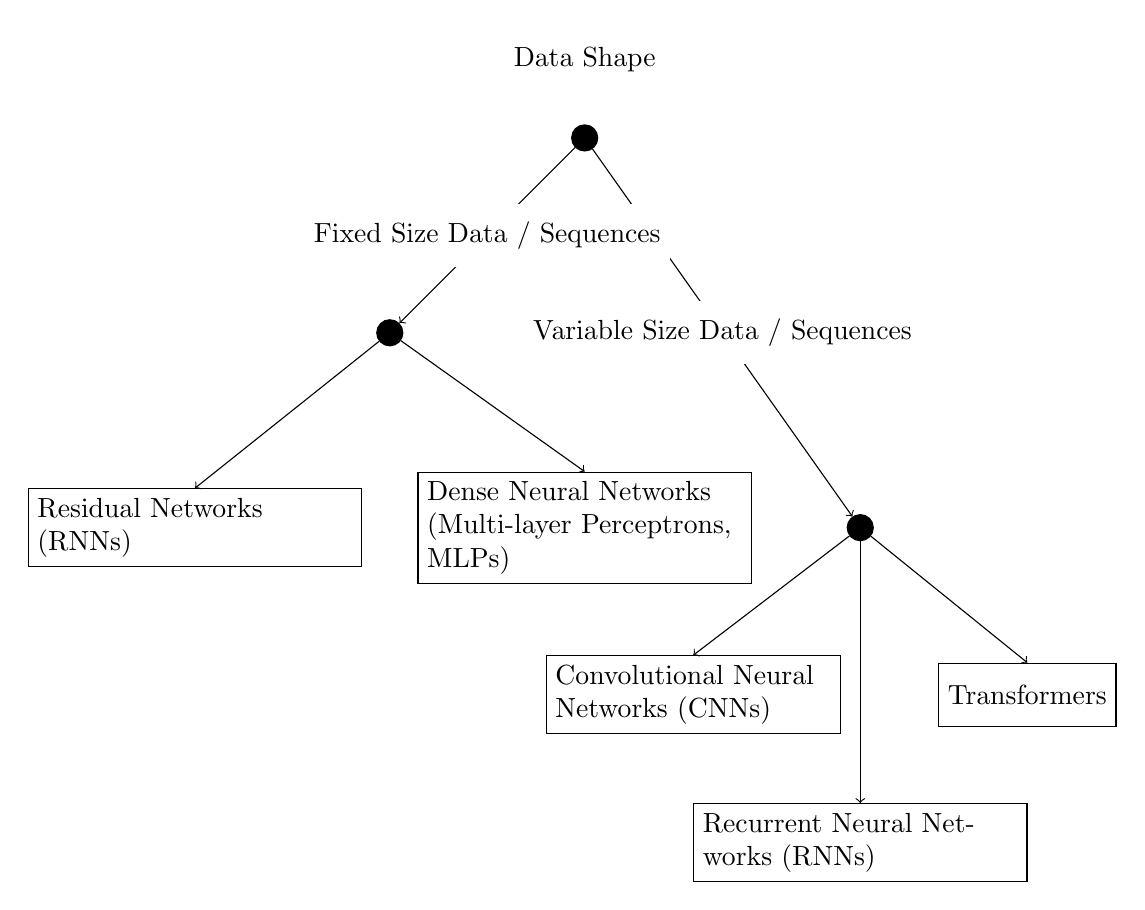
\begin{tikzpicture}
        \tikzstyle{every node}=[node distance=3.5cm,minimum height=0.8cm]
        % data shape
        \node[draw,fill=black,minimum height=0.2cm,circle] (taskroot) at (0,0) {};
        \node[above of=taskroot, node distance=1cm] {Data Shape};

        % fixed input shape
        \node[draw,fill=black,minimum height=0.2cm,circle, below left of=taskroot] (fixed)  {};

        % ResNet
        \node[draw, below left of=fixed,text width=4cm] (resnet)  {Residual Networks (RNNs)};
        \draw[->] (fixed) -- (resnet.north);

        % MLP
        \node[draw, below right of=fixed,text width=4cm] (mlp) {Dense Neural Networks (Multi-layer Perceptrons, MLPs)};
        \draw[->] (fixed) -- (mlp.north);

        % sequence
        \node[draw,fill=black,minimum height=0.2cm,circle,right of=mlp] (sequence) {};
        \draw[->] (taskroot) -- node[fill=white] {Variable Size Data / Sequences} (sequence);

        % this here to draw over above line
        \draw[->] (taskroot) -- node[fill=white] {Fixed Size Data / Sequences} (fixed);

        % CNN
        \node[draw, below left of=sequence,text width=3.5cm, node distance=3cm] (cnn) {Convolutional Neural Networks (CNNs)};
        \draw[->] (sequence) -- (cnn.north);

        % RNN
        \node[draw,below of=sequence,text width=4cm, node distance=4cm] (rnn) {Recurrent Neural Networks (RNNs)};
        \draw[->] (sequence) -- (rnn.north);

        % Transformer
        \node[draw,below right of=sequence, node distance=3cm] (transformer) {Transformers};
        \draw[->] (sequence) -- (transformer.north);

    \end{tikzpicture}
    \vspace{1cm}
    \captionsetup{parskip=7pt}
    \caption[Fixed vs variable input shape]{Neural network variants which support variable input shape.

    Due to their construction, MLPs and ResNets are restricted to a fixed input shape, and so can only be trained and used on data that is of a fixed size, such as tabular data, or data that has been processed into a fixed size by re-sampling, chunking etc.

    RNNs, CNNs and Transformers can accept variable length data, each with their own tradeoffs. They are typically more suitable for data that is naturally of variable size/length, such as text, audio or images.}
    \label{fig:ontology-input-shape}
\end{figure}

\begin{figure}
    \centering
    \begin{tikzpicture}
        \tikzstyle{every node}=[node distance=3.5cm,minimum height=0.8cm]

        % dataset type
        \node (datasettype) {Dataset Type};
        \node[draw, below of=datasettype] (seq) {Sequence Prediction};
        \draw (datasettype) -- node[fill=white] {Un-labeled} (seq);

        % input shape
        \node[right of=datasettype] (inputshape) {Data Shape};

        % loss
        \node[right of=inputshape] (loss) {Loss Functions};

        % angles
        \node[draw,fill=black,minimum height=0.2cm,circle,below of=loss,xshift=1.5cm] (angles) {};
        \draw (loss) -- node[fill=white] {Angles} (angles);

        \node[draw,fill=white,below of=angles,node distance=2.5cm, xshift=-2cm] (amse) {Squared Angular Error};
        \draw (angles) -- (amse.north);

        \node[draw,fill=white,below of=angles,node distance=2.5cm, xshift=2cm] (vonmises) {Von-Mises NLL};
        \draw (angles) -- (vonmises.north);

        \node[draw,fill=white,below of=loss,node distance=4.5cm,xshift=-1.5cm] (cat)  {Categorical};
        \draw (loss) -- node[fill=white] {Discrete} (cat.north);

        % transformer (here because needs to draw above a line)
        \node[draw, below of=inputshape] (transformer) {Transformer};
        \draw (inputshape) -- node[fill=white] {Sequences} (transformer);


        % chapter 4: arbitrary order sampling
        \node[draw,fill=white,text width=5cm] (chapter4) at (0,-8cm) {\textbf{\Cref{C:a-o-sampling}}: Arbitrary order sampling on MNIST};

        % chapter 6.2: transformer for hand pose prediction
        \node[draw,fill=white,text width=5cm] (chapter62) at (2.5cm,-10.5cm) {\textbf{\Cref{C:hand-model}, \Cref{S:mean-model}}: Predicting the next frame in a hand animation};

        % chapter 6.3: probabilistic model for hand pose prediction
        \node[draw,fill=white,text width=5cm] (chapter63) at (8cm,-10.5cm) {\textbf{\Cref{C:hand-model}, \Cref{S:prob-model}}: A flexible probabilistic model for hand motion prediction};

        \begin{pgfonlayer}{bg}
            \draw ([xshift=-4pt]seq.south) -- ([xshift=-4pt]chapter4.north);
            \draw ([xshift=-4pt]transformer.south) -- (chapter4.north);
            \draw (cat.south) -- ([xshift=4pt]chapter4.north);

            \draw (seq.south) -- ([xshift=-4pt]chapter62.north);
            \draw (transformer.south) -- (chapter62.north);
            \draw (amse.south) -- ([xshift=4pt]chapter62.north);

            \draw ([xshift=4pt]seq.south) -- ([xshift=-4pt]chapter63.north);
            \draw ([xshift=4pt]transformer.south) -- (chapter63.north);
            \draw (vonmises.south) -- ([xshift=4pt]chapter63.north);
        \end{pgfonlayer}

    \end{tikzpicture}
    \vspace{1cm}
    \captionsetup{parskip=7pt}
    \caption[Where my work sits.]{The later work in this thesis sits focuses on learning un-labeled sequence data with transformers, in two different domains.

    In \Cref{C:a-o-sampling}, I train a transformer-based probabilistic model which can be used as a gaussian process for predicting pixels on the MNIST dataset.

    In \Cref{C:hand-model}, I train a transformer-based model on the ManipNet hand motion dataset. \Cref{S:mean-model} focuses on a deterministic model, while \Cref{S:prob-model} focuses on a probabilistic model.}
    \label{fig:ontology-context}
\end{figure}

\TODO{ Use the correct terminology for " Regression (\textit{implicit} MLE)" and "Parameter regression (\textit{explicit} MLE)"}

The choice of training objective affects the settings in which a model can be used, which theoretical properties we get from it, and more.

The simplest kind of training objective is regression. When we train a model with a regression objective it learns to predict the expected value of the output. Regression is characterized by using an error function as the loss, for example \textit{mean-squared-error}:
\newcommand{\mse}{L_{\text{MSE}}}
\begin{align}
\label{notation:mse}
\begin{split}
    \fdef{\mse}{\R^{N×D}×\R^{N×D}}{\R} \\
    \mse&(y, \hat{y})_{ni} ≝ \frac{1}{N} \sum_n\left[ \sum_i (y_{ni} - \hat{y}_{ni})^2 \right]
\end{split}
\end{align}
This function sums the error over the \textit{feature} dimension $D$ and averages the error over the \textit{batch} dimension $N$ \footnote{Averaging has no effect on the optimization, it is simply that dividing by the batch and/or sequence length means that the loss value remains in the same range independent of the batch size or sequence length.}. Training a model by minimising this loss function, is equivalent to maximising the likelihood of a Gaussian distribution. Given input $x$, the model output $y = f(x)$ can be interpreted as $\E[p(y|x)]$.


\section{Auto-regressive models}

\TODO{ Formulation of auto-regressive models and sampling }

\TODO{ Things we can do with an auto-regressive model }

\section{Animation}


\section{Angle representations}

\TODO{ Quaternions and unitary / complex matrices }
